\documentclass[11pt]{article}
\usepackage{amssymb}
\usepackage{algpseudocode}
\usepackage{algorithm}
\usepackage{setspace}
\usepackage{graphicx}
\graphicspath{ {./images/} }
\usepackage{hyperref}

\hypersetup{
    colorlinks=true,
    linkcolor=blue,
    filecolor=magenta,      
    urlcolor=cyan,
}

\title{MSc Project - Binding Affinity Prediction of Protein-Ligand Complex}
\author{
        Abdus Salam Khazi\\
        \href{mailto:abdus.khazi@students.uni-freiburg.de}
                {abdus.khazi@students.uni-freiburg.de}\\ \\
        Supervisors:
        \begin{tabular}{ll}
			Simon Bray \&
			Alireza Khanteymoori
		\end{tabular}
       }
	
\begin{document}

\maketitle
\date{}
\tableofcontents
\newpage

\section{Introduction}
.....TOBE REFINED AFTER COMPLETING THE FULL REPORT.....

\subsection{Biological Background}
Proteins are the work horses of our body.
Every main function is carried out by a protein or a collection of proteins.
Ligands are molecules that bind to proteins to form protein ligand complexes.
Ligands can be molecules that the protein transports like in the case of the haemoglobin
transporter.

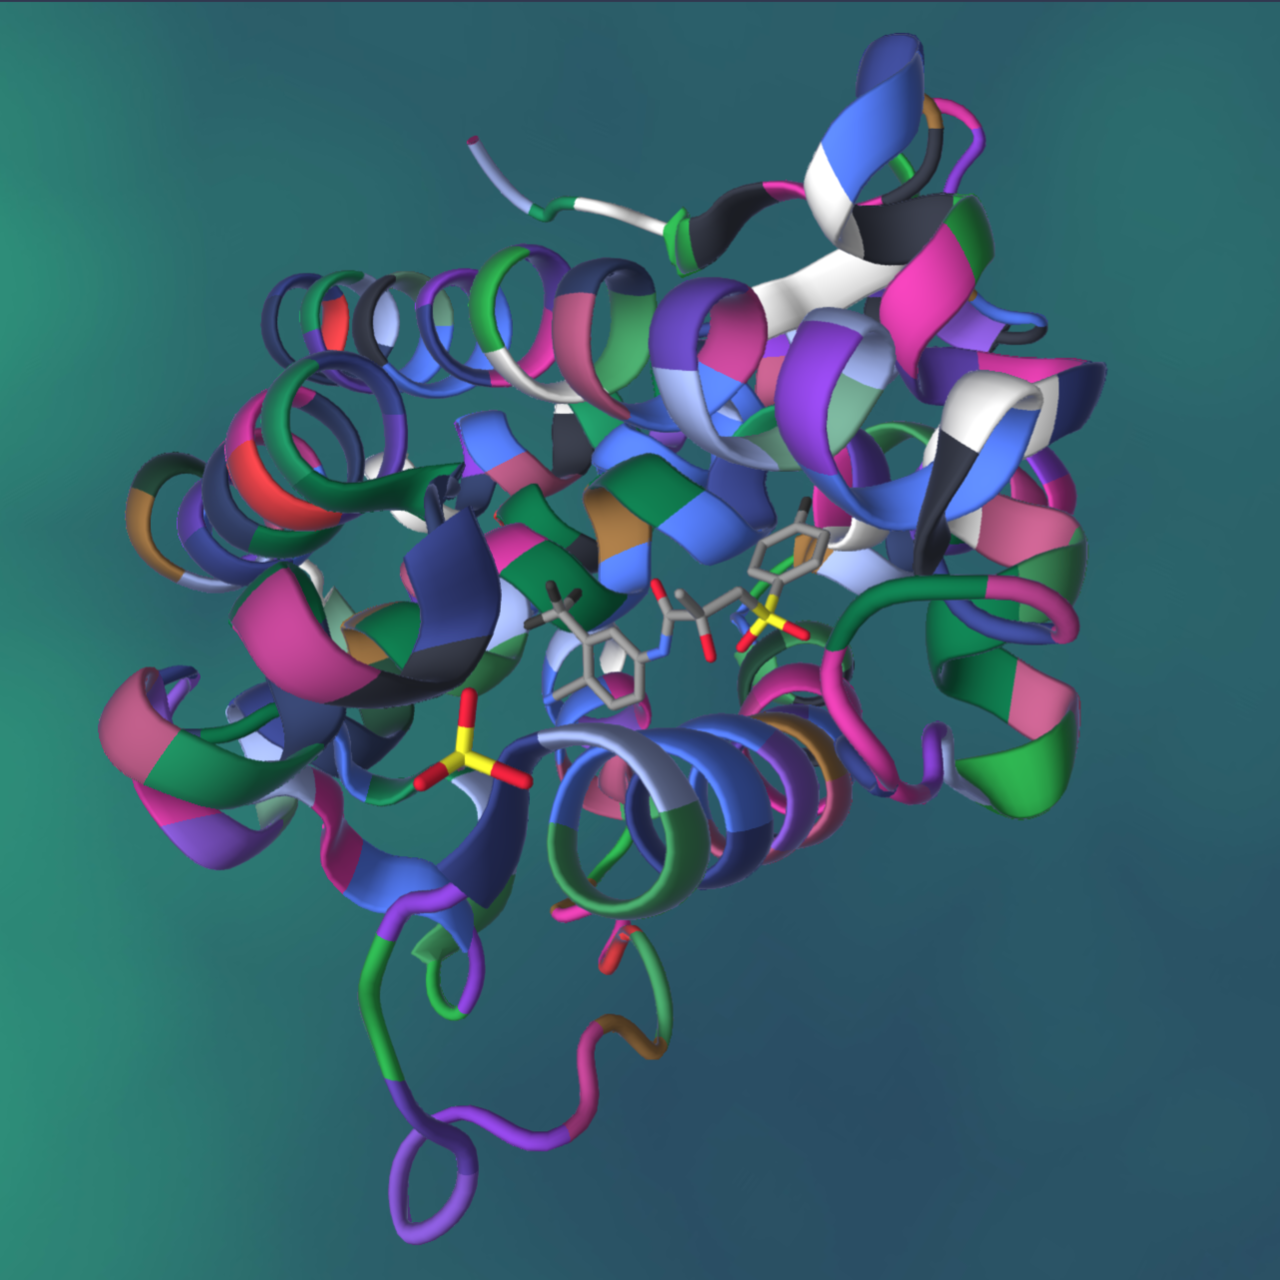
\includegraphics[scale=0.15]{pl_complex}
\cite{PL_complex_introduction}


They can also be stimulators or agents that start or stop the functioning of the protein.
When ligands and proteins bind with each other, they form a protein-ligand complex.
The correct functions of these complexes is very essential for our body.
Hence the study of this data is very helpful for biologists and bioinformaticians...

....TALK about drug discovery here ...

\subsection{Representation of molecules and complexes in the pdb bind data set}

PDB format is used to represent the protein molecules (macro molecules).
It contains information regarding the coordinates of atoms like the XYZ format in Armstrong units.
It contains information regarding protein secondary structures.
Because of the presence of 3D positional data, molecular visualization is possible using specialized software. 
The format has to be column specific if we want it to work with legacy software.
\href{https://www.youtube.com/watch?v=_1q7sfjl2Kw}{Video Link}.
\href{https://en.wikipedia.org/wiki/Protein_Data_Bank_(file_format)}{PDB format}\\

SDF format file is a type of molecular descriptive file which contains x,y,z format similar to pdb format.
It also contains bond information.
This data can be used to create a graph using which SMILES string can be created.
\href{https://en.wikipedia.org/wiki/Chemical_table_file}{SDF format}

Mol2 format file is also a file similar to the sdf format.
We chose to use this format because we could extract the features of more molecules
using this format as compared to the sdf format.

\section{Problem Formulation}
Protein-Ligand complex problems can be broadly classified into 2 types -
\begin{itemize}
\item LBS - Ligand binding site prediction.
\item Ligand affinity prediction.
\end{itemize} 

LBS (Ligand binding side) prediction can be further classified into 3 types -
\begin{itemize}
\item 3D structure based
\item Template based
\item Sequence based
\end{itemize}

The problem that we deal is Binding affinity prediction. 
The protein ligand complex binding affinity is defined by a number Kd which is called dissociation constant.
This constant is given for all pl complexes in the pdb bind dataset.
In our problem we take care of the following 2 things
\begin{itemize}
\item We do not take the features of the whole protein
but take the features of the location of the protein which binds to the ligand.
This is called a pocket.
\item We try to keep the features of proteins and ligands dintinct till the input so that we can have a plug and play sort of input for our model.
The binding affinity of any protein or ligand can be found out because of this property of our modelling.
\end{itemize}

However for this we make use of existing 3D structure based LBS tool chain called fpocket.
The reason this is helpful is because 3D structural features of proteins are very crucial for the binding between 
the proteins and ligands as proteins and ligand interactions can be considered as
machines of 2 parts interacting with each other.

\subsection{fpocket / dpocket descriptors}
We extract the features of a pocket using dpocket tool (a submodule in the fpocket toolchain).
fpocket uses veronoi tessalation (3D) to find out pockets in our protein structure.
To get the descriptors/features of the pockets at which ligands bind we use the dpocket (aka descriptors pocket).
dpocket creates 3 types of descriptors for the pockets in the protein -
\begin{itemize}
\item fpocketp.  This lists all the possible pockets (with descriptors) that could bind to ligand according to a criteria.
Multiple pockets can bind with the same ligand.
Here the descriptor called overlap maybe 100\% or less.
\item fpocketnp.  This lists all pockets (with descriptors) that are not binding according to the criteria.
\item explicitp.
This lists all the explicitly binding pocket (with descriptors).
Here the overlap feature is always 100\%.
\end{itemize}

We use both fpocketp and explicitp descriptors to train our model.
There are in total 55 descriptors in total obtained using dpocket descriptors.

\subsection{DataSet}
Protein databank has been created by experiments all around the world.
From this databank, a PBD bind dataset has been created which provides data about all the protein-ligand complexes.
In our study, we propose a method to predict the protein binding affinity of novel proteins and ligands using the data given by PBD bind dataset.

\subsection{Dichotomous problem}
Since the protein and the ligand are equally responsible for the affinity between them, our problem (also the binding site prediction problems) can be classified as a dichotomous problem in which we need data from both
the protein and the ligand.
The data if it is complementary is better for solving the problem.
The accuracy measure of the protein LBS prediction is the same as the dichotomous problems in math.

\section{feature selection}
\label{fs}
Various feature selection mechanisms were used to

\subsection{Algorithm}

\begin{algorithm}
\caption{Selection of features in our model}
\begin{algorithmic}[1]
\Procedure{SELECT\_FEATURES\_BASED\_ON\_CORRELATION\_BASED\_SELECTOR}{}
\State Todo... Complete this description
\EndProcedure
\end{algorithmic}
\end{algorithm}


\section{Discussion}


\section{Conclusion}

\bibliographystyle{plain}
\bibliography{references}

\end{document}
